\chapter{Analyse comparative des  performances}
Dans cette partie, nous analysons les résultats et performances des différentes méthodes et optimisations implémentées.

\vspace{2mm}
Pour cela, nous avons lancé des séries de tests avec 100 itérations et avec des nombres particules différents. Nous avons donc mesuré et sommé le temps concerné pour chaque itération afin d'effectuer une moyenne pour chaque nombre de particules. Pour chaque méthode, les paramètres physiques seront les mêmes. Pour les versions parallélisées, le nombre de threads utilisés est toujours fixé à $4$.

\section{Construction de l'arbre}

Les tests de parallélisation de notre algorithme de construction du $quadtree$ ont montré qu'il n'est pas parallélisable. En effet,  effectuer les insertions en parallèle engendre des erreurs lors  des calculs de force par l'utilisation de cet arbre, qui font diverger les particules. Cela pourrait s'expliquer par le fait que les insertions de particules sont dépendantes les unes des autres et ne peuvent donc être effectuées en parallèle au risque de fausser les calculs. Ainsi, pour pouvoir le paralléliser, il est nécessaire de modifier au préalable le fonctionnement de l'algorithme d'insertion.

\begin{center}
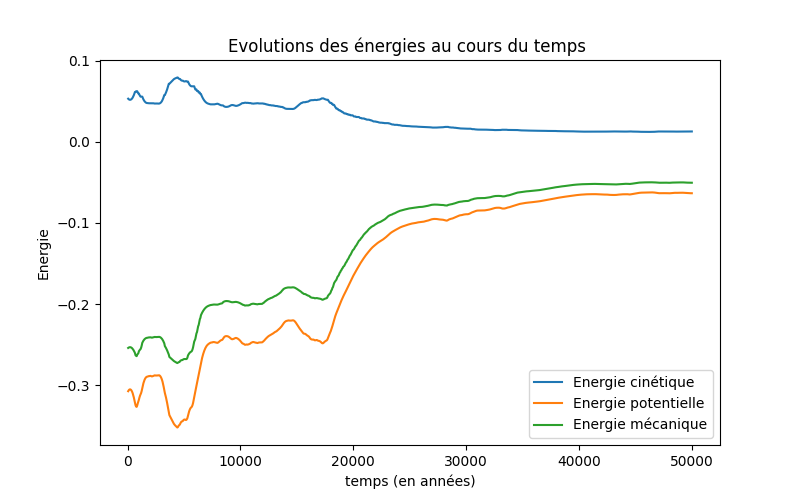
\includegraphics[scale=0.6]{./resultats/Energy_tree.png}
\captionsetup{hypcap=false}
\captionof{figure}{Bilan énergétique pour la parallélisation de la
construction de l'arbre\\
($\Delta t = 50$ ans et $1000$
itérations)}
\label{fig11}
\end{center}

On peut voir sur la figure $7.1$ que ces erreurs se traduisent simplement par l'absence de conservation de l'énergie mécanique au cours du temps, montrant ainsi que la parallélisation de la construction de l'arbre n'est pas utilisable.

\section{Comparaisons des méthodes}

\begin{minipage}[c]{.46\linewidth}
     \begin{center}
             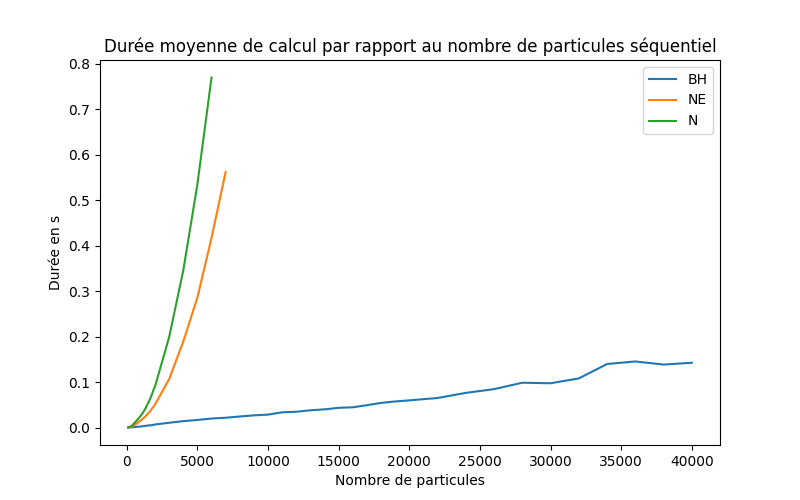
\includegraphics[width=9.5cm]{./resultats/method_comparison_seq.png}
         \end{center}
   \end{minipage} \hfill
   \begin{minipage}[c]{.46\linewidth}
    \begin{center}
     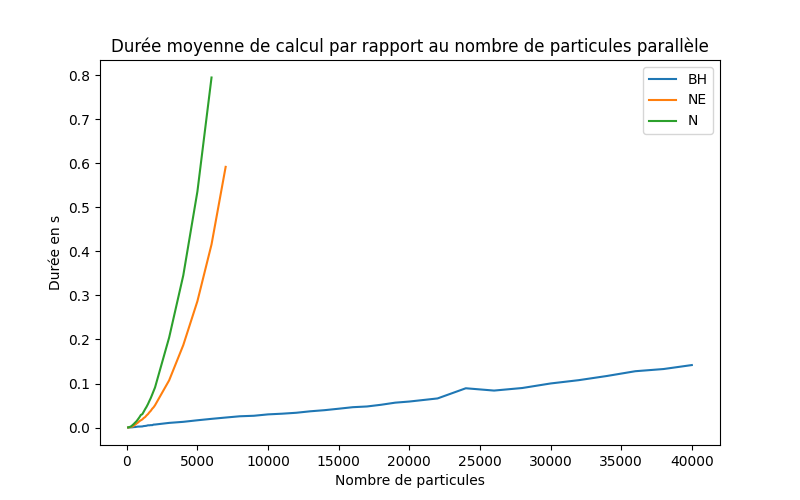
\includegraphics[width=9.5cm]{./resultats/method_comparison_par.png}
        \end{center}
 \end{minipage}
 
 \begin{center}
 \captionsetup{hypcap=false}
 \captionof{figure}{Durée moyenne en fonction du nombre de 
 particule}
\label{fig12}
 \end{center}

\par Les résultats confirment la théorie. Il est clair que les méthodes naïves ont une complexité en $O(N^2)$ alors que l'algorithme de Barnes-Hut a une complexité bien inférieure en $O(Nlog(N))$.
On peut également confirmer que l'algorithme naïf optimisé a une meilleure complexité que la version naïve.
De plus, on peut déjà remarquer que l'ordre de grandeur des durées est plus petit pour les versions parallélisées.
 
\section{Séquentiel et parallèle}

\subsection{Naïve}
\begin{center}
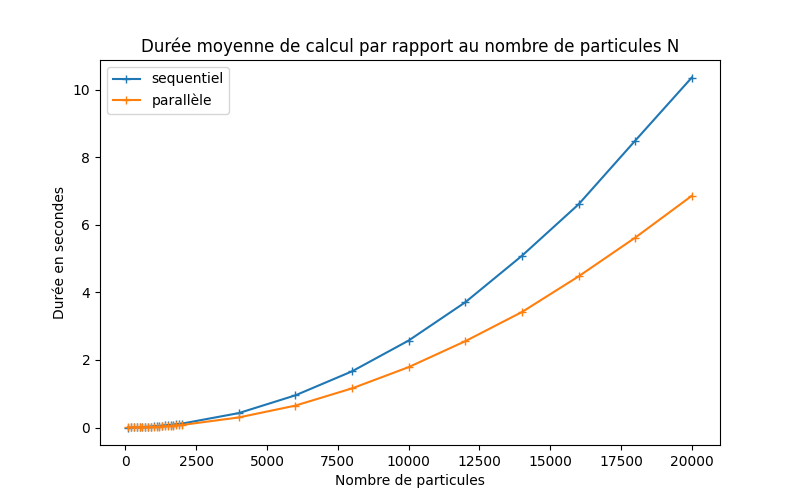
\includegraphics[scale=0.6]{./resultats/comparison_N.png}
\captionsetup{hypcap=false}
\captionof{figure}{Résultats pour l'algorithme naïf }
\label{fig15}
\end{center}


La parallélisation fonctionne bien sur la méthode de calcul naïve, le calcul parallélisé étant $1.5$ plus rapide que le calcul séquentiel. Cette amélioration n'a cependant aucun effet sur la complexité.


\subsection{Naïve optimisée}
\begin{center}
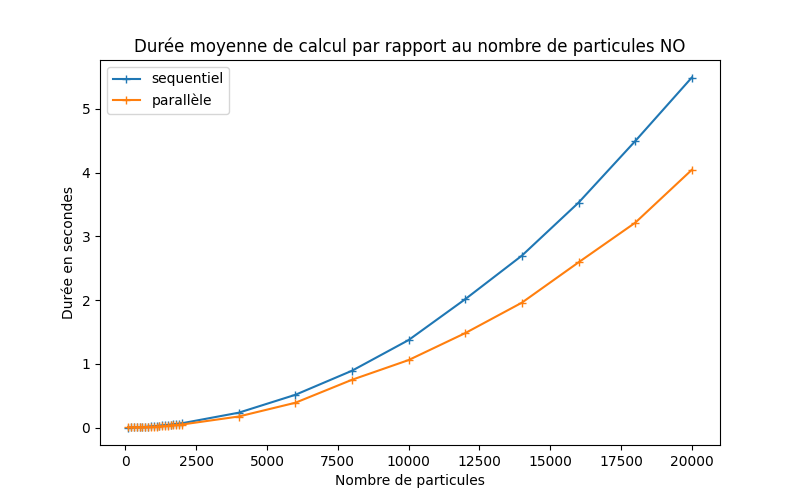
\includegraphics[scale=0.6]{./resultats/comparison_NO.png}
\captionsetup{hypcap=false}
\captionof{figure}{Résultats pour l'algorithme naïf optimisé}
\label{fig14}
\end{center}


La parallélisation fonctionne également bien sur la méthode de calcul naïve optimisée, le calcul parallélisé étant $1.4$ plus rapide que le calcul séquentiel.

\subsection{Algorithme de Barnes-Hut}
\begin{center}
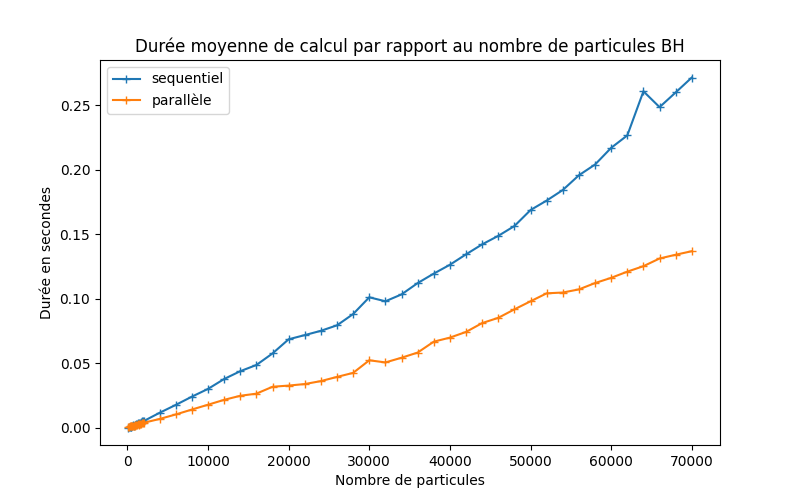
\includegraphics[scale=0.6]{./resultats/comparison_BH.png}
\captionsetup{hypcap=false}
\captionof{figure}{Résultats pour l'algorithme de Barnes-Hut}
\label{fig13}
\end{center}

On peut voir sur la figure que globalement la parallélisation améliore de manière conséquente l'efficacité des calculs de Barnes-Hut. En effet, la version parallélisée est $1.7$ fois plus rapide que la version séquentielle. Dans les deux cas la complexité est en $O(log(N))$.

\subsection{Résultats de la parallélisation}
Les résultats obtenus dans cette partie ont permis de vérifier les résultats théoriques par rapport aux performances des algorithmes : l'algorithme de Barnes-Hut est bien plus performant que les autres. De plus, ils ont également montré que la parallélisation permet bel et bien d'optimiser les calculs à conditions de respecter les conditions de parallélisation. En moyenne, le gain de vitesse avec $4$ threads est d'environ $1.53$ ce qui est plutôt élevé. Afin d'améliorer notre parallélisation, nous aurions pu augmenter le nombre de threads ou équilibrer davantage la charge entre les différents threads.